
\subsection{Recording}
The structure of a recording is restrictive in terms of arranging the components due to the design of CESAR. There are numerous ways of presenting the recording view; however, a recording structure is limited to the components of starting a recording, establishing sensor connection, monitoring of samples, and finalize sensors and recording. Additional components can be incorporated to aid a recording without causing disruption. For instance, the connectivity state component (\ref{sssec:csc}) provides extended functionality to the recording structure. In Figure \ref{fig:hta_recording}, the illustration of a recording structure with the components and their dependencies are shown:

\begin{figure}
    \centering
    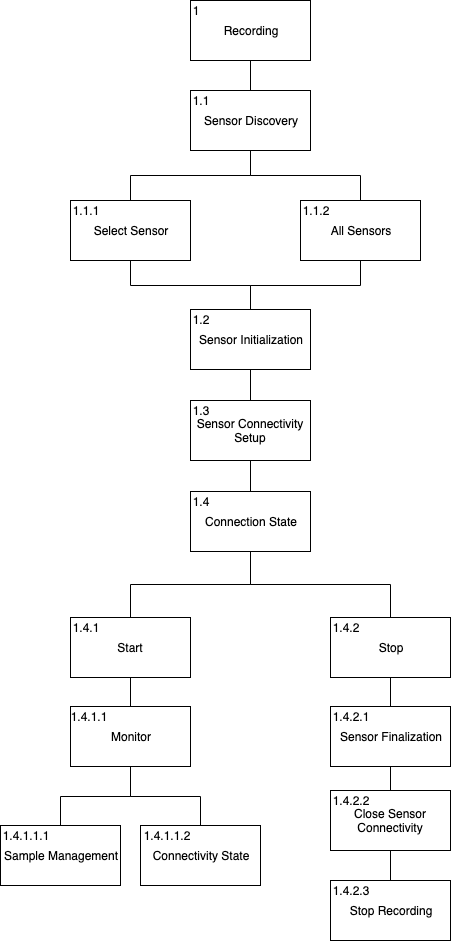
\includegraphics[width=0.5\textwidth]{images/Recording.png}
    \caption{Sharing}
    \label{fig:hta_recording}
\end{figure}

\begin{itemize}
    \item[1.1] \verb|Sensor Discover:| Has to find all eligible sensors that can enable a recording.
    \item[1.1.1] \verb|Select Sensors:| From the sensor discovery, we can choose preferable sensors sources.
    \item[1.1.2] \verb|All Sensors:| More straightforward, we sample from all of the available sensors.
    \item[1.2] \verb|Sensor Initialization:| Once we have a list of sensors sources, we need to establish and initialize a connection with the sensors. Occasionally a sensor might use some time to connect, or unforeseen occurrence is hindering the initialization of the sensor. Thus, blocking the state of the recording. 
    \item[1.3] \verb|Sensor Connectivity Setup:| Additionally, we establish a connection between the application and the sensor source. All data exchange occurs over the established interface. 
    \item[1.4] \verb|Connection Stat:| Based on sensors establishments we can proceed to either start or stop a recording. 
    \item[1.4.1] \verb|Start:| By starting, we notify the sensors to begin collecting data, and the view should display that a recording has begun accordingly.
    \item[1.4.1.1] \verb|Monitor:| Is continuously waiting for new samples to arrive on the interface defined between the application and the sensors.
    \item[1.4.1.1.1] \verb|Sample Management:| Once a new sample has arrived, we need to store the sample on a persistent storage.
    \item[1.4.1.1.2] \verb|Connectivity State:| If it is an external sensor, the sensor source might disconnect during a recording. Thus, implementing a mechanism to check for continuous data stream is a critical task.
    \item[1.4.2] \verb|Stop:| By stopping, we notify the sensors to stop collecting data from the sensor source.
    \item[1.4.2.1] \verb|Sensor Finalization:| We notify the sensor to stop sampling data, and close establishment.
    \item[1.4.2.2] \verb|Close Sensor Connectivity:| We close the interface establishment between the application and the sensors. 
    \item[1.4.2.3] \verb|Stop Recording:| Once the sensors has closed its connections, we can add additional information to the recording (e.g., title, description, rating). In the end, the recording has concluded and its stored on the mobile device.
\end{itemize}

\subsubsection{Connectivty State Component} \label{sssec:csc}
Connectivity state is a component that monitors for unexpected sensor disconnections or abruptions. Unexpected behavior can occur due to anomalies in the sensor, or the sensor being out of reach from the device for a brief moment.  A naive solution would be to ignore the connectivity state component, and assuming the sensors are connected to the device indefinitely. However, upon disconnections or abruptions, the recording would be missing samples which will result in a lacking record. This component solves the issue of missing samples by actively reconnecting the sensor based on a time interval, resulting in more accurate record with fewer gaps between samples. The following design questions for this component are 1) should the connectivity state component, which implements a time interval, be implemented in the sensor wrapper, or should it be in the proposed recording structure?; and 2) should the interval between sample arrival be a fixed time or a dynamical time? 


\begin{enumerate}
    \item To achieve a mechanism of reconnecting to the sensor on unexpected disconnects or abruptions, establishing a time interval that monitors for sample arrivals within a time frame (e.g., every 10 seconds) is required. Incorporating the time interval in the sensor wrapper reduces the complexity of Nidra. However, it introduces extra complexity to the sensor wrappers. A sensor wrapper has to distinguish actual disconnects from unexpected disconnects. Though, by extending the functionality of sensor wrapper by implementing a state that indicates whether a recording is undergoing or stopped solves the problem. All future sensor wrappers would then have to implement the proposed solution, resulting in a complicated and time-consuming sensor wrappers development. While implementing the proposed solution in the sensor wrappers is possible, extending the recording structure with the logic in Nidra would be more meaningful and time-saving. In our design, we will be implementing the connectivity state in the recording structure.
    \item A time interval triggers an event every specified time frame. If an event is triggered, a sample has not arrived, meaning the sensor either has been disconnected or abrupted. A time frame can be in a fixed size (e.g., every 10 seconds) or a dynamical size (e.g., start with 10 seconds, then incrementally increase the frame by X seconds). Implementing a fixed time frame increases the stress on put on the sensor, whereas a dynamical time might miss samples if the time frame is significant. Depending on how critical the recording is, a suitable solution for the time frame should be configurable. Also, limiting the number of attempts made to reconnect should be considered, due to actively reconnecting to a sensor that is dead or completely out of reach can cause unnecessary deterioration on the device. Thus, stopping the recording once a limited number of attempts has been reached.  In our design, we implemented a dynamical time and limited the number of attempts to 10. 
\end{enumerate}

\subsection{Sharing}

Sharing is separable into two concerns: export and import. The scope of exporting in Nidra is to select desired records, format and bundle the records into a transmittable file, and dispatching the bundle over a medium (e.g., mail). The scope of importing is to locate the file on the device, parse the content based on the format, and store it on the device. In Figure \ref{fig:hta_sharing}, the structure of sharing is presented with components and their dependencies: 

\begin{figure}
    \centering
    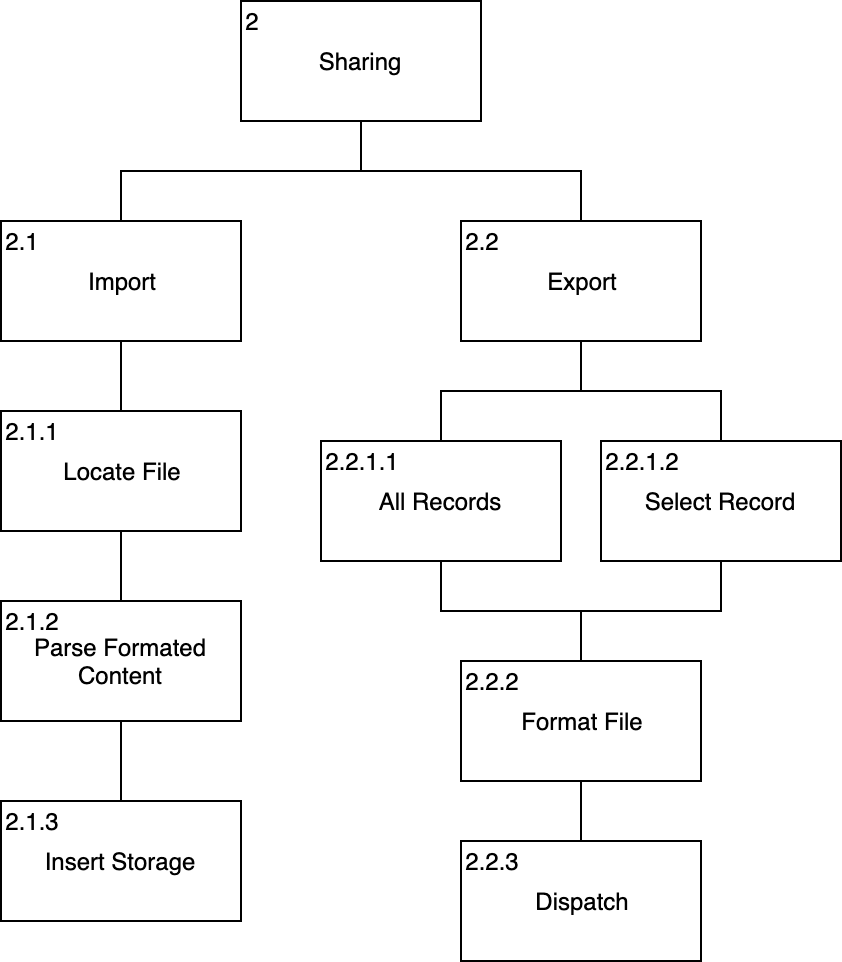
\includegraphics[width=0.5\textwidth]{images/Sharing.png}
    \caption{Sharing}
    \label{fig:hta_sharing}
\end{figure}

\begin{itemize}
    \item[2.1] \verb|Import|:
    \item[2.1.1] \verb|Locate File|: locate the file on the device.
    \item[2.1.2] \verb|Parse Formated Content|: parse the content of the file 
    \item[2.1.3] \verb|Insert Storage|: with the parsed data, insert it into the storage 
    \item[2.2] \verb|Export|:
    \item[2.2.1.1] \verb|All Records|: export all of the records on the device 
    \item[2.2.1.2] \verb|Select Record|: choose one record to export 
    \item[2.2.2] \verb|Format File|: format the records into a transmittable file  
    \item[2.2.3] \verb|Dispatch|: send the file over a medium (e.g., mail).
\end{itemize}


\subsubsection{Format File Component}

The format file component converts selected records into a formatted file. Formatting is used to serialize the data to enable transmission over the internet. Serialization is the process of converting the state of an object into a stream of bytes, which later can be deserialized by rebuilding the stream of bytes to the original object. There are several data serialization formats, and a few appropriate formats are:

\begin{itemize}
    \item \verb|JSON| is a file format used to transmit data objects consisting of attribute-value pairs and array data types [wikipedia, JSON, 9.mai]. JSON has a simple syntax, which results in a compact file and efficient transmission. However, it only supports a few data types. The markup of a JSON format is \verb|{"firstname": "Peter"}|
    \item \verb|XML| is a markup language that encodes arbitrary data structures into a format that is human-readable and machine-readable [wikipedia, XML, 9.mai]. XML provides a generalized markup that has support for numerous data types, structure validation, and extensions. However, the structure of XML results in a larger file[?]
    \item \verb|Custome Format| constructing a file format solely for transmitting records and samples - by introducing a file format that is restrictive to the purpose of records and sample, we can minimize the transmitting file size. However, this might result in unreadable text, the overhead of parsing and transforming, and incompatibilities amongst devices. 
\end{itemize}
While these format structures are applicable for transmitting data, choosing a format that is compact, human-readable, and standard format that is extensible and scalable for future data is essential. The custom format is compact, but might not be human-readable and is not a standard format. On the contrary,  JSON and XML meet these criteria the custom format is lacking. JSON in the contrast of XML is more compact and lightweight; hence, in our design, we will be using the JSON format for transmission of the data.

When a preferred format for the records is selected, bundling the data into a file for transmittal over a medium can be done. It is essential to identify the name of the file uniquely to prevent duplicates and overrides of data. For instance, it is identifying the name of the file with the device identification appended with the time of exporting. 

\subsubsection{Dispatching Component}
The dispatching component uses the formatted file and transfers it across applications. There are two distinctive methods to perform named task which is efficient and practical: 1) implement an interface with recipients to share data with, by establish a web-server with logic to handle users and sharing data with the desired recipient. Also, implementing an interface to retrieve the file within the application;  and 2) Using the interface provided by Android to share files. While the first option might be favorable in terms of practicality, this solution introduces additional concerns (e.g., the privacy matters of storing user data on a server) which is out of the scope for this project. For this reason, using the interface provided by Android is a reasonable solution. The user of the application can utilize the Android interface for sharing files over installed applications; however, e-mail is a flexible medium to transfer the file, and the user can specify the recipients accordingly.  

\subsubsection{File Location Component}
\textit{Importing} is accomplishable by locating the file, parsing the file, and storing the recordings in storage. A naive solution for the location of a file is by assuming that the file is located in on the same location amongst all devices, thus trying locating the file on a static location. Therefore, providing an interface to the users to deliberately locate the desired file in the file hierarchy of its device is practical. Android provides an interface for such a solution [?]. With the exact path of the file, we can read the bitstream of the file and parse the data according to the chosen format, and store the content of the file on the device.

\subsection{Modules}

\begin{figure}
    \centering
    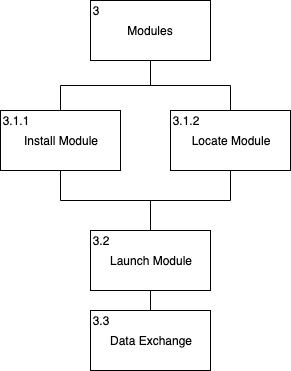
\includegraphics[width=0.3\textwidth]{images/Modules.png}
    \caption{Modules}
    \label{fig:hta_modules}
\end{figure}

Modules are independent applications that provide extended functionality and data enrichment to Nidra. The components for locating and launching a module is limited to Android design; however, the component for data exchange between a module and Nidra can be designed variously.  In Figure \ref{fig:hta_modules}, the structure of modules is presented with components and their dependencies:   

\begin{itemize}
    \item[3.1.1] \verb|Install Modules|:
    \item[3.1.2] \verb|Locate Module|: locate the file on the device.
    \item[3.2] \verb|Launch Module|: parse the content of the file 
    \item[3.3] \verb|Data Exchange|: with the parsed data, insert it into the storage 
\end{itemize}

\subsubsection{Data Exchange Component}

The data exchange component facilitates the transportation of data between Nidra and a module. As of now, the data is records and corresponding samples, which is formatted (Section Data) accordingly. The two distinct methods to exchange data between a module and Nidra are 1) formatting all of the data and bundling it into the launch of the module, and 2) establishing a communication link for pull-based requests to Nidra from the module. 

Android provides an interface to attach extra data on activity launch. The first solution is, therefore, convenient and efficient; all of the data is formatted and bundled into the launch. However, once Nidra has launched the module-application, there are no ways of transmitting new data besides relaunching the module-application. For this reason, the second option allows for continuous data flow by establishing a communication link with IPC between the applications. The data exchange between Nidra and modules can then be bidirectional; the module can request desired data any time, and Nidra can collect reports and results generated by the module. 

One could argue that new records are not obtained while managing and using a module. However, there might be future modules that do a real-time analysis of a recording; thus, require an interface for continuous data flow. For the simplicity of our design, we will be going with the first option of bundling all of the data and sending it on launch.

\subsection{Analytics}

\subsection{Storage}

\noindent Storage is the objective of achieving persistent data; data that is available after application termination.  To enable storage, we can use a database for a collection of related data that is easily accessed, managed, and updated [Database Systems, p. 52]. Three distinguishable databases structures are:
\begin{itemize}
    \item Flat file - encode a database model (e.g., table) with a collection of records without any structured relationship, in a plain text or binary file [system nosql analysis]. 
    \item Relational Database - consists of relations between data stored in tables; supporting complex queries, database transactions, and   Additionally, ensuring ACID (atomicity, consistency, isolation, and durability) properties for reliable database transactions. 
    \item Non-Relational Database - While these database structures are applicable to achieve persistent data storage, using relational database is suitable for our test
\end{itemize}

The placement of storage can be located externally on a server or internally on the device. External storage provides larger storage capacity, in addition to faster computing power. Facilitating external storage can be accomplished with maintaining a server, or utilizing a cloud service (e.g., Google Cloud) for the purpose. Internal storage provides limited storage capacity and computing power, however, the storage and retrieval data is efficient.  While both are applicable, the internal storage is more than efficient for the application.

Two distinguishable methods of structuring a storage 
There are several methods of structuring the storage on, and two distinguishable methods are a flat file or a database management system (hereafter, DBMS). File storage is a bare minimum structure of storing and retrieving data. The data is stored, with a format (e.g., JSON), in a raw file. Retrieving data occurs by reading the whole file into memory, parsing the data and then operating on the data.


\subsection{Presentation}
